\documentclass[a4paper,11pt]{scrartcl}
\usepackage[utf8x]{inputenc}
\usepackage[catalan]{babel}
\usepackage{titlesec}
% A ses llengües llatines, el primer paràgraf ha d'anar tabulat
\usepackage{indentfirst}
\usepackage{amsmath}
\usepackage{float}
\usepackage{graphicx}
\usepackage{subfigure}
\usepackage{booktabs}
\usepackage{multirow}
\usepackage{hyperref}
\usepackage{url}
\usepackage{multirow}
\usepackage{minted} %wget http://minted.googlecode.com/hg/minted.sty

% aptitude install texlive-fonts-extra
\usepackage{newcent} %font mes wapa

\graphicspath{{diagrames/}}

% Estil de seccions
\titleformat{\section}{\large\sectfont}{\thesection}{1em}{}
\titleformat{\subsection}{\bfseries\sectfont}{\thesubsection}{1em}{}
% Estil numeracio subseccions http://help-csli.stanford.edu/tex/latex-sections.shtml#number
%\def\thesubsection{\alph{subsection})}

\title{Visió per Computador}
\author{ Bartomeu Miró Mateu \thanks{bartomeumiro a gmail punt com} \\
	 Lluis Cortès Rullan \thanks{lluisbinet a gmail punt com} }

\begin{document}

  \maketitle

  \begin{abstract}
    Documentació de le sis pràctiques de l'assignatura Visió per Computador,
optativa de l'Enginyeria Informàtica impartida a la UIB.

  \end{abstract}

  \newpage
  \setcounter{page}{2}
  \tableofcontents
  \newpage

  \section{Introducció}
  Tal i com es demana de cada pràctica hi ha un petit informe, per tal de no tenir
molts fitxers dispersos aquest document els aglutina a tots ells.

  Cal esmentar que a mesura que avancen les pràctiques minvava el temps
per realitzar-les degut a l'acumulació de pràctiques d'altres assignatures.
  Així doncs no és d'estranyar que en les primeres hi hagi opcionals o funcionalitats
que no demanava l'enunciat i que a mesura que s'avança es vagin senyint més a l'enunciat.

  Un altre punt a tenir amb compte és que les pràctiques s'han desenvolupat emprant el
llenguatge de programació \emph{Python}. El motiu es que es molt més versàtil, senzill
i fàcil de emprar que no pas \emph{C++} a més de també tenir \emph{bindings}\footnotemark per \emph{OpenCV}.
Per contra partida no es té suport del professor
i sovint els exemples trobats per internet en \emph{C++} no són directament aplicables, 
cosa no suposa un problema si s'enten el que s'està fent.

No obstant recomanam l'ús de Python als altres alumnes així com a suggerencia al
professor. El fet de ser programari lliure fa que sigui de fàcil distribució i
insta\lgem ació. Per altra banda al ser un lleguatge interpretat no es requereix
fer una compilació, així doncs quan es modifica el codi en mode asseig error
no s'ha d'esperar el temps de compilació.

Esperem es tengui en compte el fet d'haver emprat un altre llenguatge suposant
un inconvenient al no poder intercanviar directament codi amb els companys i
haver demostrat més eteniment de les llibreries \emph{OpenCV} al no poder aplicar
directament \emph{copy\&paste} dels exemples que es troben \emph{on-line}.

\footnotetext{\url{http://opencv.willowgarage.com/documentation/python/index.html}}

%   \include{p1/doc/p1-doc}
%   \include{p2/doc/p2-doc}
%   \include{p3/doc/p3-doc}
%   \include{p4/doc/p4-doc}
%   \include{p5/doc/p5-doc}
%   \include{p6/doc/p6-doc}

%% Peu de pàgina.
 \let\thefootnote\relax\footnotetext{
 Aquest document està baix llicència \href{http://creativecommons.org/licenses/by-sa/3.0/}{Creative Commons Atributive Share-Alike 3.0}
 per tant es pot compartir, modificar i distribuir, però citant els autors 
 originals i sense modificar la llicència.
 De la mateixa manera el codi font està baix llicència GNU GPL v3 per part
 dels dos autors.\bigskip}

\let\thefootnote\relax\footnotetext{El document en versió digital i el codi
 font el trobareu a \\ \url{https://github.com/bmiro/vpc}\bigskip}

\let\thefootnote\relax\footnotetext{Aquest document i tota la
 pràctica ha estat desenvolupat emprant programari lliure o codi obert:}

\let\thefootnote\relax\footnotetext{\href{http://www.tug.org/applications/pdftex/}{\LaTeX}
 i \href{http://www.tug.org/applications/pdftex/}{Kile} per el text,
\href{http://www.inkscape.org/}{Inkscape} pels diagrames,
\href{http://kate-editor.org/}{Kate} i \href{http://vim.org/}{Vim} per l'edició del codi font.
\href{http://git-scm.com/}{Git} com a sistema de control de versions,
\href{http://python.org}{Python} com a llenguatge de programació 
amb les llibrereis \href{http://opencv.willowgarage.com/wiki/}{OpenCV}.

}

\let\thefootnote\relax\footnotetext{
\begin{center}
\begin{tabular}{cc}

\includegraphics[height=35pt,keepaspectratio=true]{diagrames/by-sa.png}
 & 
\includegraphics[height=35pt,keepaspectratio=true]{diagrames/gnu.png}
\end{tabular}
\end{center}

\begin{center}
\begin{tabular}{ccccc}
 
\includegraphics[height=35pt,keepaspectratio=true]{diagrames/latex.png}
 & 
\includegraphics[height=35pt,keepaspectratio=true]{diagrames/kile.png}
 & 
\includegraphics[height=35pt,keepaspectratio=true]{diagrames/inkscape.png}
 & 
\includegraphics[height=35pt,keepaspectratio=true]{diagrames/vim.jpg}
 & 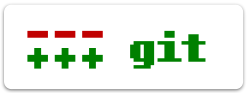
\includegraphics[height=35pt,keepaspectratio=true]{diagrames/git.png}
\end{tabular}
\end{center}

\begin{center}
\begin{tabular}{cc}
  
\includegraphics[height=35pt,keepaspectratio=true]{diagrames/python.png}
 & 
\includegraphics[height=35pt,keepaspectratio=true]{diagrames/opencv.png}
\end{tabular}
\end{center}
}

\end{document}
